\chapter{L'intégration numérique}\label{chap-quadrature}

La MEF discrétisant une formulation faible,  la construction des matrices 
constitutives du système à  résoudre comportent dont des intégrations.

Dans certains cas particuliers, ou en utilisant des codes de calcul formel, ces intégrations
peuvent être réalisées de manière exactes.

Mais, dans la plupart des cas (et dans la plupart des codes de calcul), ces
intégrations sont calculées numériquement. On parle alors de méthodes
d'intégration numérique et de formules de quadrature.






\medskip
\section{Méthode de Newton-Cotes}\index[aut]{Cotes (Roger), 1682-1716, Anglais}\index[aut]{Newton (Isaac, Sir -), 1643-1727, Anglais}\index{Méthode de Newton-Cotes}

Soit à calculer l'intégrale suivante:
\begin{equation}I=\int_a^b f(x)dx\end{equation}

\medskip
L'idée consiste à construire un polynôme pour interpoler $f(x)$, et
à intégrer ce polynôme.

\medskip
Plusieurs types de polynômes peuvent être utilisés pour cette interpolation.
Les principales méthodes d'interpolations sont détaillées au chapitre \ref{chap-interpolation}.



\medskip
\subsection*{Méthode des rectangles}\index{Méthode des rectangles}

La \textcolorblue{méthode des rectangles} consiste à interpoler $f(x)$ par un
polynôme de degré $0$, i.e. par la constante valant, selon les variantes de la
méthode, soit $f(a)$, soit $f((a+b)/2)$.

\medskip
Comme cette approximation est très brutale, il est possible de subsiviser
l'intervalle $[a,b]$ en plusieurs intervalles et d'appliquer la méthode sur chacun
des intervalles, i.e. d'approcher $f$ par une fonction en escalier.

Si l'on subsivise l'intervalle $[a,b]$ en $n$ intervalles égaux, il vient alors:
\begin{equation}I\approx h\sum_{i=0}^{n-1} f(x_i)\end{equation}
où $h=(b-a)/n$ est la longueur de chaque sous intervalle et $x_i=a+ih$ le
point courant.




\medskip
\subsection*{Méthode des trapèzes}\index{Méthode des trapèzes}

La \textcolorblue{méthode des trapèzes} consiste à interpoler $f(x)$ par un polynôme 
de degré $1$, i.e. par la droite passant par les points $(a,f(a))$ et $(b,f(b))$.
On obtient alors:
\begin{equation} I\approx h\dfrac{f(a)+f(b)}2\end{equation}
où $h=b-a$ est la longueur de l'intervalle,
et l'erreur commise vaut $-\frac{h^3}{12} f''(w)$ pour un certain $w\in[a,b]$
(sous réserve que $f$ soit 2 fois dérivable).

L'erreur étant proportionnelle à $f''$, la méthode est dite d'ordre $2$, ce qui
signifie qu'elle est exacte (erreur nulle) pour tout polynôme de degré inférieur
où égale \ a 1.

\medskip
Comme cette approximation peut sembler un peu brutale, il est possible de subsiviser
l'intervalle $[a,b]$ en plusieurs intervalles et d'appliquer cette formule sur chacun
des intervalles, i.e. d'approcher $f$ par une fonction affine continue par morceaux.

Si l'on subsivise l'intervalle $[a,b]$ en $n$ intervalles égaux, il vient alors:
\begin{equation}I\approx \frac{(b-a)}{n}\sum_{i=0}^{n}f(x_i)\end{equation}
où $h=(b-a)/n$ est la longueur de chaque sous intervalle, $x_i=a+ih$ le
point courant et l'erreur commise vaut $-\frac{h^3}{12n^2} f''(w)$ pour un certain $w\in[a,b]$.

\medskip
\textbf{Remarques:}
\begin{itemize}
\item la \textcolorblue{méthode de Romberg}\index[aut]{Romberg (Werner), 1909–2003, Allemand}, publiée en 1955,
(elle même basée sur le procédé d'extropolation de Richardson)\index[aut]{Richardson (Lewis Fry), 1881-1953, Anglais}
permet d'accélérer la convergence de la méthode des trapèze (Wiki est ton ami).
\item La méthode des trapèzes est un cas particulier de celle de Newton-Cotes pour $n=1$.\index[aut]{Cotes (Roger), 1682-1716, Anglais}\index[aut]{Newton (Isaac, Sir -), 1643-1727, Anglais}\index{Méthode de Newton-Cotes}
\end{itemize}

\medskip
\subsection*{Méthode de Simpson}\index{Méthode de Simpson}\index[aut]{Simpson (Thomas), 1710-1761, Anglais}

La \textcolorblue{méthode de Simpson}  consiste à interpoler $f(x)$ par un polynôme 
de degré $2$, i.e. par la parabole passant par les points extrêmes $(a,f(a))$ et $(b,f(b))$ 
et le point milieu $(c,f(c))$ avec $c=(a+b)/2$.
On obtient alors:
\begin{equation} I\approx \frac{h}{6} \left( f(a)+f(b)+f(c)\right)\end{equation}
où $h=b-a$ est la longueur de l'intervalle,
et l'erreur commise vaut $-\frac{h^5}{2^5.90} f^{(4)}(w)$ pour un certain $w\in[a,b]$
(sous réserve que $f$ soit 4 fois dérivable).

L'erreur étant proportionnelle à $f^{(4)}$, la méthode est dite d'ordre $4$, ce qui
signifie qu'elle est exacte (erreur nulle) pour tout polynôme de degré inférieur
où égale \ a 3.

\medskip
Comme dans le cas préc\'edent, il est possible de subsiviser l'intervalle $[a,b]$ en plusieurs intervalles 
et d'appliquer cette formule sur chacun des intervalles.

Si l'on subsivise l'intervalle $[a,b]$ en $n$ intervalles égaux, avec $n$ pair, il vient alors:
\begin{equation} I\approx \frac{h}{3} \left( f(a)+f(b)+2\sum_{i=1}^{n/2-1}f(x_{2i})+4\sum_{i=1}^{n/2}f(x_{2i-1})
\right)\end{equation}
où $h=(b-a)/n$ est la longueur de chaque sous intervalle, $x_i=a+ih$ le
point courant et l'erreur commise vaut $-\frac{nh^5}{180} f^{(4)}(w)$ pour un certain $w\in[a,b]$.

\medskip
\textbf{Remarques:}
\begin{itemize}
\item La parabole interpolant $f$ est trouvée en utilisant l'interpolation de Lagrange.\index[aut]{Lagrange (Joseph Louis, comte de -), 1736-1813, Italien}
\item La méthode de Simpson\index[aut]{Simpson (Thomas), 1710-1761, Anglais} est un cas particulier de 
	celle de Newton-Cotes pour $n=2$.\index[aut]{Cotes (Roger), 1682-1716, Anglais}\index[aut]{Newton (Isaac, Sir -), 1643-1727, Anglais}\index{Méthode de Newton-Cotes}
\end{itemize}


\medskip
\subsection*{Méthode de Newton-Cotes}\index[aut]{Cotes (Roger), 1682-1716, Anglais}\index[aut]{Newton (Isaac, Sir -), 1643-1727, Anglais}\index{Méthode de Newton-Cotes}

Les \textcolorblue{formules de Newton-Cotes} se proposent également d'approximer
l'intégrale $I$ et découpant l'intervalle $[a,b]$ en $n$ intervalles identiques.
On posera donc encore une fois $h=(b-a)/n$ la longueur de chaque sous intervalle, 
et $x_i=a+ih$ le point courant.
La formule est:
\begin{equation} I\approx \sum_{i=0}^n \varpi_i f(x_i) \end{equation}
où les $\varpi_i$ sont appelés \textcolorblue{poids} ou \textcolorblue{coefficients
de la quadrature} et sont construits à partir des polynômes de Lagrange.

\medskip
\textcolorblue{La méthode de Newton-Cotes intègre exactement un polynôme de degré $n-1$ 
avec $n$ points.}

\medskip
\textbf{Remarque:}
Il est possible de construire une formule de Newton-Cotes de degré quelconque.
Toutefois, une telle formule \textcolorred{n'est pas inconditionnellement stable.}

C'est pourquoi, on se cantonnera aux plus bas degrés:
$n=0$ méthode du point médian (i.e. méthode des rectangle où la valeur est
évaluée en milieu d'intervalle); 
$n=1$ méthode des trapèzes;
$n=2$ méthode de Simpson dite 1/3, i.e. celle présenntée avant;
$n=3$ méthode de Simpson 3/8 (il suffit de faire le calcul);
$n=4$ méthode de Boole.

Lorsque le degré augmente, des instabilités apparaissent, dues au
\textcolorblue{phénomène de Runge}.\index[aut]{Runge (Carl David Tolmé), 1856-1927, Allemand}
En effet, avec certaines fonctions (même infiniment dérivables), l'augmentation 
du nombre $n$ de points d'interpolation ne constitue pas nécessairement une bonne 
stratégie d'approximation.
Carle Runge a montré qu'il existe des configurations où l'écart maximal entre la fonction 
et son interpolation augmente indéfiniment avec $n$.
Pour remédier à cela on peut utiliser les abscisses de Tchebychev\index[aut]{Tchebychev (Pafnouti Lvovitch), 1821-1894, Russe} 
au lieu de points équirépartis pour interpoler, ou plus simplement utiliser des splines (i.e. des polynômes 
par morceaux), et donc augmenter le nombre de morceaux et non le degré des polynômes.








\medskip
\section{Méthodes de quadrature de Gauss}\index[aut]{Gau\ss{} (Johann Carl Friedrich), 1777-1855, Allemand}\index{Méthode de quadrature de Gau\ss{}}

Le principe de la méthode reste le même que pour la méthode de Newton-Cotes, mais
on va essayer d'améliorer un peu encore la qualité du résultat.
Pour cela, on souhaite que:
\begin{equation}I=\int_a^b \varpi(x)f(x)dx \approx \sum_{i=1}^n \varpi_if(x_i)\end{equation}
où $\varpi(x): (a,b)\rightarrow\RR$ est une \textcolorblue{fonction de pondération}, 
qui peut assurer l'intégrabilité de $f$. 
Les $\varpi_i$ sont appelés les \textcolorblue{poids ou coefficients de quadrature (ou poids)}.
Les $x_i$ sont réels, distincts, uniques et sont les racines de polynêmes orthogonaux 
(et non plus uniquement de Lagrange) pour le produit scalaire 
$\left\langle f,g \right\rangle = \int_a^b f(x)g(x) \varpi(x) \,\mathrm{d}x$. 
Ils sont appelés  \textcolorblue{points ou nœuds de Gauss}.
Les poids et les nœuds sont choisis de façon à obtenir des degrés d'exactitude les plus 
grands possibles.
Cette fois-ci \textcolorred{$(a,b)$ peut être n'importe quel type d'intervalle (fermé, ouvert, fini ou non).}

\medskip
\subsection*{Intégration sur un intervalle type}\index{Polynôme! orthogonalité}\index{Polynôme! de Legendre}\index{Polynôme! de Tchebychev}\index{Polynôme! d'Hermite}\index{Polynôme! de Laguerre}\index[aut]{Laguerre (Edmond Nicolas), 1834-1886, Français}\index[aut]{Legendre (Adrien-Marie), 1752-1833, Français}\index[aut]{Hermite (Charles), 1822-1901, Français}\index[aut]{Tchebychev (Pafnouti Lvovitch), 1821-1894, Russe}


\begin{center}
\begin{tabular}{lll}
Intervalle $(a,b)$ & Fonction de pondération $\varpi(x)$ & Famille de polynômes orthogonaux\\
\hline
$[-1,1]$ & $1$ & Legendre\\
$]-1,1[$ & $(1-x)^\alpha (1+x)^\beta \ , \ \alpha, \beta > -1$ & Jacobi\\
$]-1,1[$ & $\frac{1}{\sqrt{1-x^2}}$ &Tchebychev (premier type)\\
$]-1,1[$ & $\sqrt{1-x^2}$ & Tchebychev (second type)\\
$\RR^+$ & $\mathrm{e}^{-x}$ & Laguerre\\
$\RR$ & $\mathrm{e}^{-x^2}$ & Hermite\\
\end{tabular}
\end{center}

On rappelle que les nœuds sont déterminés comme les $n$ racines du $n$ème 
polynôme orthogonal associé à la formule de quadrature.

\medskip
\textcolorblue{Les méthodes de quadrature de Gauss intègrent exactement un polynôme de degré $2n-1$ 
avec $n$ points.}\index[aut]{Gau\ss{} (Johann Carl Friedrich), 1777-1855, Allemand}\index{Méthode de quadrature de Gau\ss{}}

\medskip
\subsection*{Changement d'intervalle d'intégration}

Si on intègre sur $(a,b)$ au lieu de $(-1,1)$, alors on fait un changement de
variable.
Finalement, on obtient l'approximation:
\begin{equation}   \frac{b-a}{2} \sum_{i=1}^n \varpi_i f\left(\frac{b-a}{2}x_i + \frac{a+b}{2}\right)  \end{equation}

\medskip
\textbf{Remarques:}
\begin{itemize}
\item \textcolorred{Pour la MEF, l'intégration se déroule sur l'élément de référence, donc on n'a
pas besoin de faire ce changement (il est fait par la transformation affine entre l'élément
considéré et l'élément de référence).}
\item Le nombre de points de Gauss\index[aut]{Gau\ss{} (Johann Carl Friedrich), 1777-1855, Allemand} ainsi que leurs positions sur l'élément sont donnés dans 
les documentations des logiciels \textcolorgris{(mais vous n'en avez maintenant plus besoin, vous savez
les trouver...)}.
\end{itemize}

\begin{figure}[ht]
\begin{center}
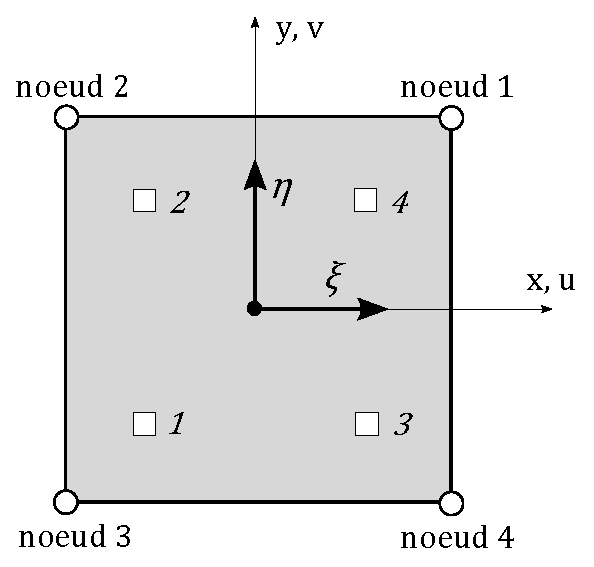
\includegraphics[height=50mm]{ptGauss.eps}
\end{center}
\caption{\label{ptGauss} Éléments rectangulaire $Q$1 de référence avec ces 4 points de Gauss (petits carrés)}
\end{figure}

\medskip
\subsection*{Intégration sur des carrés ou des cubes}

Sur les carrés et les cubes (qui correspondent à ce qui nous intéresse en terme
d'\{eléments de référence), on obtient les formules suivantes:
\begin{equation} \int_{-1}^{-1}\int_{-1}^{-1} f(x,y)dxdy \approx
\dsum_{i=1}^{n_x}\dsum_{j=1}^{n_y} \varpi_i\varpi_j f(x_i,x_j)\end{equation}

\begin{equation} \int_{-1}^{-1}\int_{-1}^{-1}\int_{-1}^{-1} f(x,y,z)dxdydz \approx
\dsum_{i=1}^{n_x}\dsum_{j=1}^{n_y}\dsum_{k=1}^{n_z} \varpi_i\varpi_j\varpi_k f(x_i,x_j,x_k)\end{equation}
où $n_x$, $n_y$ et $n_z$ sont les nombres de points de Gauss utilisés dans
les directions $x$, $y$ et $z$.

Dans la pratique, on a souvent $n_x=n_y=n_z$.


\medskip
\subsection*{Intégration sur un triangle ou un tétraèdre}

Malheureusement, tous les éléments ne sont pas des segments, carrés ou cubes...
on a également souvent à faire à des triangles et à des tétreèdres.

Dans ce cas, on construit des formules spécifiques qui ne sont pas issues du cas 1D.

L'élément triangulaire de référence est un triangle isocèle côtés égaux
de longueur 1. L'angle droit est à l'origine du repère. La forme générale d'intégration est:
\begin{equation}
I=\int_{\hat{K}} f(x,y)dxdy \approx \sum_{i=1}^n \varpi_if(x_i,y_i)
\end{equation}

\medskip
Les positions et poids des $n$ points de Gauss\index[aut]{Gau\ss{} (Johann Carl Friedrich), 1777-1855, Allemand} 
sont choisis afin d'intégrer exactement un polynôme de degré $N$.

Il vient:
\begin{center}
\begin{tabular}{cccccc}
 & $n$ & $x_i$ & $y_i$ & $\varpi_i$ & $N$\\
\hline
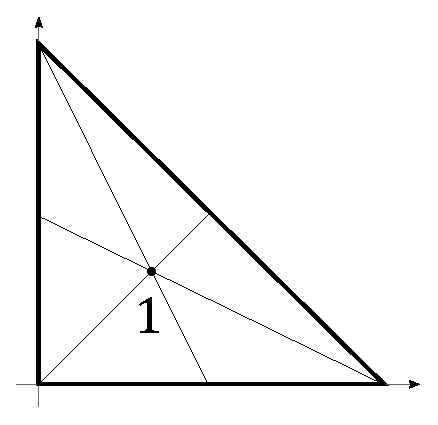
\includegraphics[height=20mm]{trG1.eps} & 1 & 1/3 & 1/3 & 1/2 & 1\\
\hline
\multirow{3}{*}{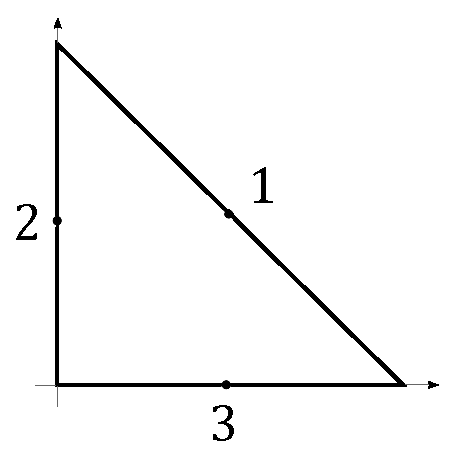
\includegraphics[width=20mm]{trG2.eps}} &
\multirow{3}{*}{3} & 1/2 & 1/2 & \multirow{3}{*}{1/6} & \multirow{3}{*}{2}\\[+2mm]
&&0&1/2&&\\[+2mm]
&&1/2&0&&\\[+2mm]
\hline
\multirow{3}{*}{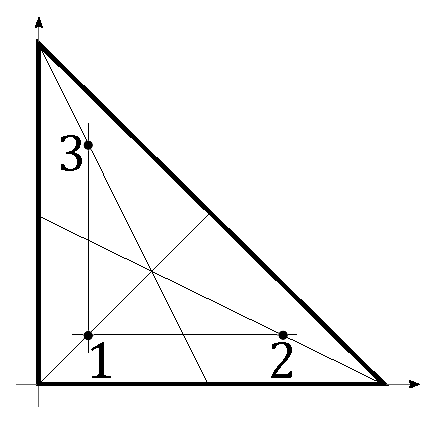
\includegraphics[height=20mm]{trG3.eps}} &
\multirow{3}{*}{3} & 1/6 & 1/6 &  \multirow{3}{*}{1/6} & \multirow{3}{*}{2}\\[+2mm]
&&2/3 & 1/6 &&\\[+2mm]
&&1/6&2/3&&\\[+2mm]
\\
\hline
\multirow{4}{*}{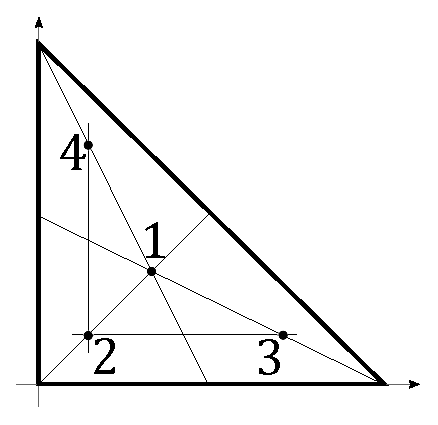
\includegraphics[height=20mm]{trG4.eps}} & 
\multirow{4}{*}{4} & 1/3 & 1/3 & -27/96 & \multirow{3}{*}{4}\\[+2mm]
&&1/5&1/5&25/96&\\[+2mm]
&&3/5&1/5&25/96&\\[+2mm]
&&1/5&3/5&25/96&\\[+2mm]
\end{tabular}
\end{center}

\medskip
Le même travail peut être fait sur un tétraèdre.


%\medskip
%\section{Condensation statique}
%
%La condensation statique a déjà été présentée dans le cadre du développement
%de super-éléments.
%
%Nous avons mentionné d'ailleurs qu'un élément peut être considéré en lui-même 
%comme un super-élément.
%
%La méthode de condensation statique peut donc lui être appliquée.

